\documentclass[a4paper, 14pt]{extarticle}
\input{../../.preambles/10-russian}
\input{../../.preambles/20-math}
\usepackage[utf8]{inputenc}
\usepackage[paper=a4paper, top=1cm, right=1cm, bottom=1.5cm, left=2cm]{geometry}
\usepackage{setspace}
\usepackage{ifthen}
\usepackage{array}
\usepackage{bm}
\onehalfspacing

\usepackage{graphicx}
\graphicspath{{plots/}, {images/}}

\parindent=1.25cm

\renewcommand{\thesection}{\arabic{section}.}
\renewcommand{\thesubsection}{\arabic{section}.\arabic{subsection}.}
\numberwithin{equation}{section}

\usepackage{caption}
\DeclareCaptionLabelFormat{figure}{Рисунок #2}
\DeclareCaptionLabelFormat{table}{Таблица #2}
\DeclareCaptionLabelSeparator{sep}{~---~}
\captionsetup{labelsep=sep,justification=centering,font=small}
\captionsetup[figure]{labelformat=figure}
\captionsetup[table]{labelformat=table}

\usepackage{titlesec}
\titleformat{\section}
    {\centering\normalsize\bfseries}
    {\thesection}
    {1em}{}
\titleformat{\subsection}
    {\normalsize\bfseries}
    {\thesubsection}
    {1em}{}

% Настройка вертикальных и горизонтальных отступов
\titlespacing*{\section}{\parindent}{*4}{*4}
\titlespacing*{\subsection}{\parindent}{*4}{*4}

\usepackage[square, numbers, sort&compress]{natbib}
\makeatletter
\bibliographystyle{unsrt}
\renewcommand{\@biblabel}[1]{#1.} 
\makeatother
\addto\captionsrussian{\def\bibname{Список использованных источников}}
\addto\captionsrussian{\def\refname{Список использованных источников}}

\newcolumntype{C}[1]{>{\centering\arraybackslash}m{#1\textwidth}}
\renewcommand{\arraystretch}{1.2}

\usepackage{color}
\definecolor{darkgreen}{rgb}{0,.5,0}
\usepackage[colorlinks,linkcolor=black,filecolor=blue,citecolor=darkgreen,urlcolor=black]{hyperref}

\newcommand{\maketitlepage}[1]{
    \begin{titlepage}
        \singlespacing
        \newpage
        \begin{center}
            Министерство образования и науки Российской Федерации \\
            Федеральное государственное бюджетное образовательное \\
            учреждение высшего профессионального образования \\
            <<Волгоградский государственный технический университет>> \\
            Факультет электроники и вычислительной техники \\
            Кафедра физики
        \end{center}
        \vspace{9em}
        \begin{center}
           { \large\bfseries ОТЧЕТ }
            \\ О научно-исследовательской практике на \( \underset{\text{наименование организации}}{\rule{.35\textwidth}{.5pt}\hrulefill} \)
        \end{center}
        \vspace{4em}
        \begin{table}[h!]
            \center         
            \begin{tabular}{b{.3\textwidth}ccl}
                Руководитель практики от организации & \( \underset{\text{должность}}{\rule{3cm}{.5pt}\hrulefill} \) & \( \underset{\text{подпись}}{\rule{3cm}{.5pt}\hrulefill} \) & Виснер~С.~В. \\
                Руководитель практики от университета & доцент & \( \underset{\text{подпись}}{\rule{3cm}{.5pt}\hrulefill} \) & Поляков~И.~В. \\
                Студент группы Ф-369 & \multicolumn{2}{c}{\( \underset{\text{подпись}}{\rule{6.5cm}{.5pt}\hrulefill} \)} & #1
            \end{tabular}
        \end{table}
        \vspace{5em}

        \begin{flushright}
            \begin{minipage}{.5\textwidth}
                Отчет защищен с оценкой \hrulefill
            \end{minipage}
        \end{flushright}
        \vspace{\fill}
        \begin{center}
            Волгоград, \the\year
        \end{center}

    \end{titlepage}
    \setcounter{page}{2}
}


\begin{document}
\maketitlepage{Чечеткин~И.~А.}
\setcounter{page}{3}
\section*{Аннотация}

В данной работе приведены цели и задачи научно-исследовательской практики, а
также описаны принципы проектирования импульсного источника питания (за основу
взят источник питания на 12 вольт). Приведено краткое описание прохождения
практики (электрическая схема блока питания, описание практической части).

\section*{Список ключевых понятий}

Трансформатор, viper, диодный мост, SMD-монтаж, дроссель, индуктивность,
рассеиваемая мощность, накопительный конденсатор.
\newpage

\tableofcontents
\newpage

\phantomsection\addcontentsline{toc}{section}{Введение}
\section*{Введение} Прохождение практики студентами на предприятии подразумевает
собой ознакомление студентов с реальным технологическим процессом и закреплением
теоретических знаний, полученных в ходе обучения.
	
На протяжении долгого времени остается актуальным вопрос о производстве
различных источников питания, ведь от них зависит нормальное функционирование
бытовых электроприборов. Каждый год рынок предлагает большое разнообразие
подобной продукции, имеющую различные входные и выходные характеристики,
соответствующие спросу потребителей. К ним относятся источники питания для
мобильных устройств, силовая электроника, различные инверторы напряжения и т.~п.
На основе изученной литературы и рынка выпускаемой продукции, была проведена
подготовительная работа, связанная с решением поставленной задачи. За основу
блока питания была использована схема обратноходового преобразователя.
	
Преобразователь с передачей энергии на обратном ходу (обратноходовой
преобразователь, \emph{Flyback}, флайбэк) можно назвать одной из самых
популярных топологий импульсных источников питания.

Основное преимущество обратноходовой топологии~-- дешевизна и малое количество
деталей. Поэтому практически все сетевые источники питания до мощностей
30--50~Вт строятся именно по этой топологии. Флайбэк прекрасно справляется с
формированием нескольких выходных напряжений с неплохой стабильностью
дополнительных напряжений, не требуя при этом практически никаких
схемотехнических изысканий. \newpage

\section{Принцип действия обратноходового преобразователя и основные
соотношения для расчета}
\begin{figure}[h!]
	\center
	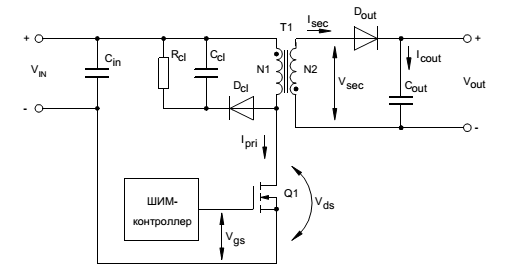
\includegraphics[width=.6\textwidth]{m_01}
	\parbox{.6\textwidth}{\caption{Силовая часть обратноходового
	преобразователя}\label{p01}}
\end{figure}
На рис.~\ref{p01} изображена силовая часть обратноходового преобразователя, а на
рис.~\ref{p02}~-- диаграммы его основных токов и напряжений.
		
\begin{figure}[h!]
	\begin{minipage}{.5\textwidth}
		Будем анализировать самый распространенный режим работы~-- режим
		разрывных токов (\emph{discontinuous}). Это значит, что к началу
		следующего цикла вся энергия из трансформатора передана в нагрузку, и
		следующий цикл начинается с нулевого тока в трансформаторе. Режим
		безразрывных токов (\emph{continuous}) распространен гораздо меньше.
		
		Для анализа разобьем рабочий цикл на отдельные периоды. Пусть схема
		работает на частоте \( f \), при этом период будет \( T = 1/f \).
		Интервал \( t_0 - t_1 \)~-- время включенного состояния силового ключа
		\( Q_1 \) (время прямого хода)~-- обозначим как \( t_{ON} \),
		соответственно рабочий цикл (\emph{Duty Circle}, в дальнейшем \( D \))
		будет определяться как \( D = t_{ON}/T \).
			 
		\textbf{Интервал \( \bm{t_0 - t_1} \).} К моменту \( t_0 \) сердечник
		трансформатора полностью размагничен, и ток в нем отсутствует. В момент,
		когда с ШИМ-контроллера подается управляющий сигнал, силовой
	\end{minipage} \hfill
	\begin{minipage}{.45\textwidth}
		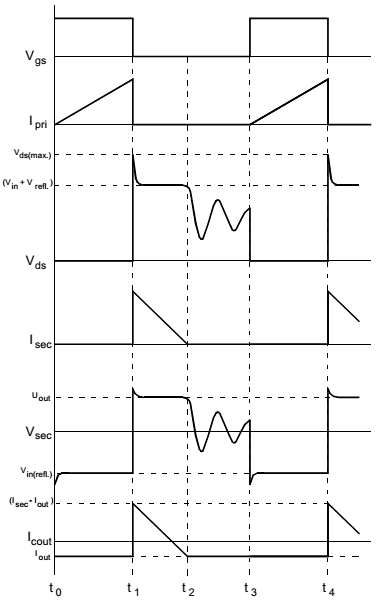
\includegraphics[width=\textwidth]{m_02}
		\parbox{\textwidth}{\caption{Диаграммы токов и напряжений
		обратноходового преобразователя}\label{p02}}
	\end{minipage}
\end{figure}
\noindent ключ \( Q_1 \) открывается и ток в трансформаторе начинает нарастать.

То есть в идеализированной схеме включение силового транзистора происходит при нулевом
токе. В реальных же условиях происходит некоторый бросок тока, связанный с
зарядом паразитных емкостей трансформатора, что при больших входных напряжениях
приводит к существенным потерям в ключе и возникновению паразитных
высокочастотных колебаний. Для уменьшения последних стремятся несколько
замедлить процесс открывания транзистора для уменьшения паразитных токов.
Выходной диод также полностью закрыт к этому времени, и нет необходимости в
быстром его перезаряде/восстановлении.

Ток в индуктивности первичной обмотки трансформатора \( L_{PRI} \) будет
нарастать до тех пор, пока ШИМ-контроллер не даст команду на выключение силового
транзистора. ШИМ-контроллер рассчитывает (исходя из сигнала рассогласования
обратной связи) количество энергии, которую необходимо запасти для поддержания
постоянной мощности в нагрузке плюс потери в самом источнике. Если мощность в
нагрузке обозначить как \( P_{OUT} \), то за время прямого хода мы должны
запасти следующее количество энергии:
\begin{equation}
	A = \frac{P_{OUT}}{\eta\cdot f},
\end{equation}
где \( \eta \)~-- коэффициент полезного действия (КПД), \( f \) -- частота
преобразования.

Энергия, запасаемая в индуктивности есть
\begin{equation}
	A = \frac{L\cdot I_{PRI}^2}{2},
\end{equation}
и можно найти ток, который нарастет в первичной обмотке трансформатора за время
прямого хода:
\begin{equation}
	I = \sqrt\frac{2\cdot A}{L_{PRI}} = \sqrt\frac{2\cdot P_{OUT}}
	{\eta\cdot f\cdot L_{PRI}}.
\end{equation}
Для определения необходимой индуктивности первичной обмотки будет
использоваться это соотношение совместно с формулой:
\begin{equation}
	U = L\cdot\der{I}{t}.
\end{equation}

Величина импульсного тока не зависит от входного напряжения~-- это позволяет
строить прекрасно работающие на практике схемы ограничения выходного тока
(точнее, выходной мощности).

Теперь следует узнать среднеквадратичное значение первичного тока~-- это
необходимо для расчета потерь в силовом ключе и в обмотке трансформатора. Для
тока пилообразной формы среднеквадратичное его значение будет:
\begin{equation}
	I_{RMS} = I_{PRI}\cdot\sqrt\frac{D}{3}.
\end{equation}
Соответственно, статические потери в силовом ключе будут:
\begin{equation}
	P_{DC} = I_{RMS}^2\cdot R_{DC},
\end{equation}
где \( R_{DC} \)~-- сопротивление канала открытого транзистора.

Потери в первичной обмотке в общем случае считаются с учетом эффекта близости.

На вторичной обмотке во время этого интервала ток нагрузки поддерживается
исключительно выходным конденсатором. К выходному диоду \( \mathrm{D_{OUT}} \)
приложено трансформированное входное напряжение. Если первичная обмотка содержит
\( N_1 \) витков, а вторичная~-- \( N_2 \), то коэффициент трансформации
\begin{equation}
	K = \frac{N_1}{N_2},
\end{equation}
и обратное напряжение на диоде \( \mathrm{D_{OUT}} \) есть:
\begin{equation}
	V_{D_{OUT}} = \frac{V_{IN}}{K} + (V_{OUT} + V_D),
\end{equation}
где \( V_D \)~-- прямое падение напряжения на выходном диоде.

При использовании диодов Шоттки с недостаточным запасом по напряжению в этом
интервале могут возникнуть проблемы~-- при большом напряжении обратный ток диода
Шоттки может достигать существенных значений~-- единиц и даже десятков
миллиампер, что вкупе с большим обратным напряжением создает большую
рассеиваемую мощность, особенно при повышенной температуре~-- здесь можно легко
получить потери превышающие даже потери от протекания прямого тока.

\textbf{Интервал \( \bm{t_1 - t_2} \)}.

Силовой транзистор выключается, ток в нем резко спадает от \( I_{PRI} \) до
нуля, а напряжение начинает быстро расти и достигает \( V_{MAX} \). Можно
ожидать, что в этот момент происходит большое выделение энергии от динамических
потерь. К сожалению, оценить их достаточно сложно, слишком много параметров
влияет на скорость этого процесса, и влияние времени переключения весьма и
весьма высоко. В общем случае:
\begin{equation}
	P_{SW} = \frac{I_{PRI}\cdot V_{MAX}\cdot t_{SW}\cdot f}{2}.
\end{equation}
		
\begin{figure}[h!]
	\begin{minipage}{.5\textwidth}
		Интервал времени \( t_{SW} \) зависит от энергии переключения силового
		транзистора, суммарного сопротивления в цепи его затвора, напряжения
		питания выходного каскада драйвера, индуктивности в цепи истока. Но
		первичный ток также начинает перезаряжать паразитную емкость
		трансформатора, снижая скорость нарастания напряжения на ключе. Этот
		эффект снижает динамические потери (а иногда вообще может свести их
		влияние к нулю). Поэтому влияние динамических потерь оказывается
		гораздо более существенным для \emph{DC-DC}~конверторов с их низкими
		входными напряжениями, большими первичными токами и высокими частотами
		преобразования, а в сетевых источниках становятся существенными потери
		от перезаряда паразитной емкости:
		\begin{equation}
			P_{SW,\,CAP} = \frac{C_p\cdot V_{SW}^2\cdot f}{2}.
		\end{equation}
	\end{minipage} \hfill
	\begin{minipage}{.45\textwidth}
		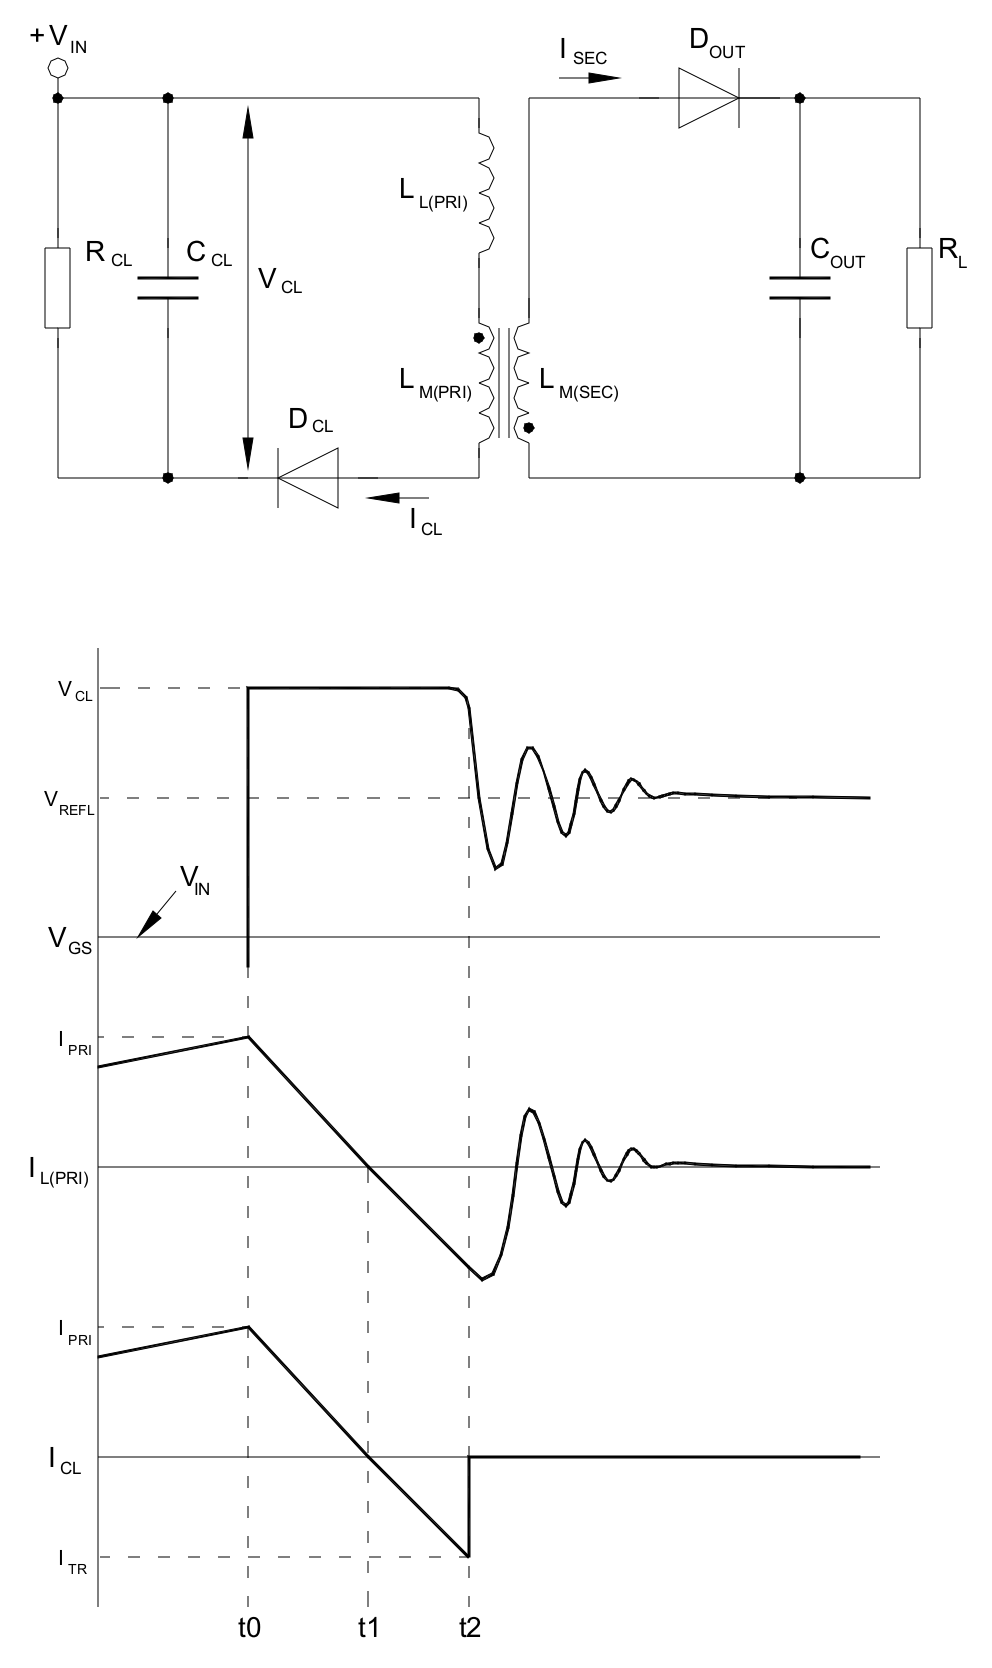
\includegraphics[width=\textwidth]{m_03}
		\parbox{\textwidth}{\caption{Часть схемы и ее диаграммы токов и
		напряжений, участвующей в выключении транзистора}\label{p03}}
	\end{minipage}
\end{figure}

Если бы трансформатор был бы идеальным, то напряжение \( V_{DS\,(MAX)} \)
равнялось бы выходному напряжению умноженному на коэффициент трансформации
(\( V_{REFL} \)). Но, к сожалению, наличие паразитных элементов схемы, в
основном индуктивности рассеяния трансформатора, приводит к существенному
выбросу напряжения на разомкнувшемся силовом ключе. Механизм образования этого
выброса неочевиден, и заслуживает подробного рассмотрения.
		
Рассмотрим вариант использования наиболее распространенного \emph{RCD}~демпфера.
Возможен вариант, когда элементы \( \mathrm{R_{CL}} \) и \( \mathrm{C_{CL}} \)
заменяются на TVS (\emph{Transient Voltage Suppressor})~-- разновидность
стабилитрона с высоким напряжением и большой поглощаемой энергией.
		
В трансформаторе обратноходового преобразователя существуют две паразитные
индуктивности, не связанные с основным потоком, и, строго говоря, правильнее
будет рассматривать процессы на модели идеального трансформатора с вынесенными
индуктивностями рассеяния первичной и вторичной стороны.

Ограничимся тем, что приведем их к одной индуктивности \( \mathrm{L_{L(PRI)}} \)
на первичной стороне~-- математические выражения для описания работы демпфера
будут теми же самыми. На рис.~\ref{p03} показана часть схемы, участвующая в
процессе выключения силового транзистора с диаграммами токов и напряжений в
некоторых точках. Мы считаем, что емкость конденсатора демпфера
\( \mathrm{C_{CL}} \) достаточно велика, чтобы пренебречь пульсациями напряжения
на нем.

Итак, в момент \( t_0 \) силовой ключ разомкнулся, и ток в первичной цепи
начинает спадать. Это вызывает мгновенный реверс напряжения на всех обмотках
трансформатора, напряжение на первичной обмотке идеального трансформатора
оказывается зафиксированным на уровне выходного напряжения, т.е. \( V_{REFL} \),
соответственно, к индуктивности рассеяния приложено напряжение
\( V_{CL} - V_{REFL} \). В момент \( t_0 \) ток в индуктивности рассеяния равен
току намагничивания, т.е. \( I_{PRI} \), и спадает до нуля за время \( t_{CH} \):
\begin{equation}
	t_{CH} = \frac{L_{L(PRI)}\cdot I_{PRI}}{V_{CL} - V_{REFL}}.
\end{equation}

Этот линейно спадающий ток втекает в конденсатор демпфера \( C_{CL} \), заряжая
его. Удобно оперировать средним его значением:
\begin{equation}
	I_{CH} = I_{PRI}\cdot\frac{D}{2} = \frac{I_{PRI}\cdot t_{CH}\cdot f}{2} =
	\frac{I_{PRI}^2\cdot L_{L(PRI)}\cdot f}{2\cdot (V_{CL} - V_{REFL})}.
\end{equation}

Как только ток в паразитной индуктивности спал до нуля, напряжение на ней пропало и, 
соответственно, напряжение на силовом ключе тоже пытается опуститься до уровня
\( V_{REFL} \). Если бы диод \( \mathrm{D_{CL}} \) был идеальным, переходный
процесс оказался бы законченным~-- энергия в индуктивности рассеяния первичной
обмотки равна нулю, а в индуктивности рассеяния вторичной обмотки~-- току
намагничивания, и демпфер полностью отключен от остальных цепей. Но
высоковольтные диоды обладают весьма существенным временем восстановления,
обычно начиная от десятков наносекунд, и здесь мы вынуждены с ним считаться. К
счастью, в данном случае это время играет положительную роль~-- на практике даже
часто стараются использовать диоды с относительно большим временем
восстановления, это значительно снижает напряжение на демпфере и,
соответственно, потери в нем.

Итак, в момент \( t_1 \) напряжение на индуктивности рассеяния через не
закрывшийся диод все еще поддерживается на уровне \( V_{CL} - V_{REFL} \), и
ток в ней начинает нарастать по закону:
\begin{equation}
	I_{LL(PRI)} = \frac{(V_{CL} - V_{REFL})\cdot t}{L_{L(PRI)}}.
\end{equation}

Если приведенные индуктивности рассеяния первичной и вторичной обмоток равны, то
этот ток, через магнитное поле трансформатора складывающийся с током вторичной
обмотки, в точности компенсирует уменьшение тока намагничивания, и ток,
поступающий в нагрузку и в конденсатор \( \mathrm{C_{OUT}} \), оказывается
постоянным на время восстановления обратного сопротивления диода демпфера. То
есть в интервале \( t_1 - t_2 \) происходит передача энергии из конденсатора
демпфера в нагрузку.

К сожалению, время восстановления обратного сопротивления диода мы можем только
оценить~-- в документации эта величина приводится для постоянного обратного
тока. В нашем случае линейно нарастающего тока она будет несколько больше, и
<<медленный>> диод восстанавливает свое сопротивление достаточно медленно, но
для оценки будем оперировать заявленной величиной.

За время \( t_{RR} \) ток в индуктивности рассеяния достигнет величины
\begin{equation}
	I_{LL(PRI)} = \frac{(V_{CL} - V_{REFL})\cdot t_{RR}}{L_{L(PRI)}},
\end{equation}
и среднее его значение за период составит:
\begin{equation}
	I_{RR} = \frac{I_{LL(PRI)}\cdot D}{2} = \frac{(V_{CL} - V_{REFL})\cdot t_{RR}^2
	\cdot f}{2\cdot L_{L(PRI)}}.
\end{equation}

В момент \( t_2 \) диод \( \mathrm{D_{CL}} \) восстановил свое сопротивление,
ток в индуктивности \( \mathrm{L_{L(PRI)}} \) начинает осциллировать по
спадающей синусоиде в резонансном контуре, образованному индуктивностью
рассеяния первичной обмотки и паразитной емкостью трансформатора, и на процессы
в демпфере уже никакого влияния не оказывает. Теперь конденсатор
\( \mathrm{C_{CL}} \) разряжается лишь током через резистор
\( \mathrm{R_{CL}} \), а поскольку пульсации на нем пренебрежимо малы, то:
\begin{equation}
	I_{DCH} = \frac{V_{CL}}{R_{CL}}.
\end{equation} 
 
Теперь известны все токи через конденсатор \( \mathrm{C_{CL}} \), и из условия
постоянного на нем напряжения можем сказать что:
\begin{equation}
	I_{CH} = I_{DCH} + I_{RR}.
\end{equation}
 
При использовании <<быстрого>> диода демпфера влияние времени его восстановления не 
очень существенно, а при использовании <<медленного>> диода даже оценить время его 
восстановления очень сложно, поэтому пренебрежем током \( I_{RR} \): 
\begin{equation}
	\frac{I_{PRI}^2\cdot L_{L(PRI)}\cdot f}{2\cdot (V_{CL} - V_{REFL})} =
	\frac{V_{CL}}{R_{CL}},
\end{equation}
откуда можно найти необходимое значение сопротивления резистора
\( \mathrm{R_{CL}} \) для получения желаемого напряжения на демпфере:
\begin{equation}
	R_{CL} = \frac{2\cdot V_{CL}\cdot (V_{CL} - V_{REFL})}
	{I_{PRI}^2\cdot L_{L(PRI)}\cdot f}.
\end{equation}
 
На практике это означает, что вычисленное значение будет минимальным, и влияние
времени восстановления диода демпфера только увеличит его значение. При
использовании <<медленного>> диода приходится эмпирически подбирать значение
\( R_{CL} \). Мощность, рассеиваемая на резисторе демпфера будет:
\begin{equation}
	P_{RCL} = \frac{V_{CL}^2}{R_{CL}}.
\end{equation}
 
Если мы используем TVS в качестве демпфера, то время восстановления диода
демпфера уже не помогает~-- TVS не способен запасать энергию и, соответственно,
отдавать ее в нагрузку. Поэтому мощность на нем будет равна произведению
среднего тока, втекающего в демпфер, на напряжение \( V_{CL} \) (и,
соответственно, напряжению срабатывания TVS):
\begin{equation}
	P_{TVS} = \frac{I_{PRI}^2\cdot L_{L(PRI)}\cdot f}{2\cdot(V_{CL} - V_{REFL})}
	\cdot V_{CL}.
\end{equation}

Поскольку в момент \( t_1 \) ток в индуктивности рассеяния оказался равным нулю,
и TVS мгновенно закрылся, не происходит дальнейшего накопления энергии, и
осцилляции напряжения на индуктивности рассеяния гораздо ниже, чем в
RCD~демпфере.

\section{Схема и выбор компонентов}

\begin{figure}[ht]
	\center
	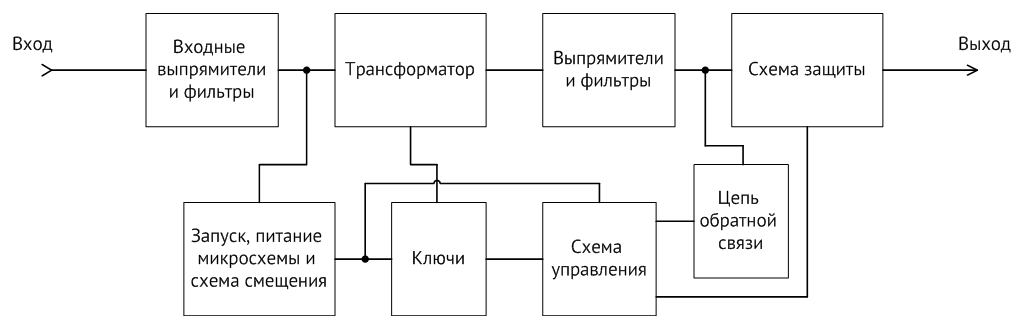
\includegraphics[width=.65\textwidth]{m_04}
	\caption{Функциональная блок-схема}\label{p04}
\end{figure}

На рис.~\ref{p04} приведена функциональная блок-схема импульсного источника
питания, на основе которой было проведено дальнейшее построение электрической 
схемы обратноходового преобразователя (рис.~\ref{p05}), базируемого на
микросхеме \emph{Viper53}. Данная схема очень удобна для рассмотрения общих
схемотехнических принципов, которые легко могут быть применены и в большинстве
других случаев.

\begin{table}[h!]
	\center
	\caption{Входные и выходные характеристики} \label{t01}
	\begin{tabular}{|*{6}{C{.15}|}} \hline
		Входное напряжение & Выходное напряжение & Выходной ток & Выходная мощность &
		Частота преобразования & КПД \\ \hline
		220~VAC \( \pm 20\% \) & 12~VDC & 0,6~А & 7,2~Вт & 100~кГц & 80~\% \\ \hline
	\end{tabular}
\end{table}

На основе предыдущего параграфа, а также с помощью использования следующих
программ: \emph{Flyback}, \emph{Viper Flyback} и \emph{Lite-CalcIT} (2000),
имея входные и выходные данные была разработана и рассчитана схема импульсного
блока питания на 12~В, применяемого для светодиодной схемы мощностью 7~Вт.
Номиналы и наименования всех элементов приведены в таблице~\ref{t02}.

\begin{figure}[ht]
	\center
	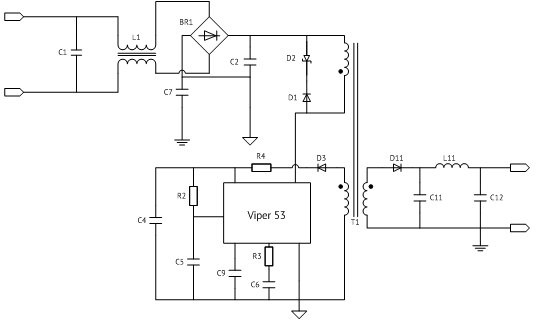
\includegraphics{m_05}
	\caption{Электрическая схема}\label{p05}
\end{figure}

\begin{table}[h!]
	\center
	\caption{Номиналы и наименования элементов электрической схемы} \label{t02}
	\begin{tabular}{|*{14}{C{.05}|}} \hline
		\multicolumn{2}{|C{.1}|}{C1} & C2 & C4 & C5 & C6 & \multicolumn{2}{C{.1}|}{C7}
		& C9 & C11 & C12 & R2 & R3 & R4 \\ \hline
		\multicolumn{2}{|C{.1}|}{22 мкФ -- 1~кВ} & 10 мкФ & 4,7 мкФ & 2,2 нФ & 47 нФ
		& \multicolumn{2}{C{.1}|}{2,2 нФ -- 2~кВ} & 22 нФ & 0,33 мФ & 56 мкФ & 6,8 кОм
		& 820 Ом & 10 Ом \\ \hline
	\end{tabular}
	\begin{tabular}{|*{3}{C{.079}|}*{3}{C{.1}|}C{.15}|C{.11}|} \hline
		L1 & L11 & T1 & D1 & D2 & D3 & D11 & BR1 \\ \hline
		6,8 мкГн & 10 мкГн & 1,35 мГн & BYT11 & BZW04-188 & BAS21 & STPS1H100 &
		KC407A \\ \hline
	\end{tabular}
\end{table} 


\section{Практическая часть}
В данной работе был собран импульсный блок питания для светодиодной схемы. В
работе была использована печатная плата, нелинейные элементы (конденсаторы,
резисторы и~т.~п.), трансформатор (расчет трансформатора осуществлен через
приведенные ранее программы).

Помимо сборки электрической схемы была поставлена задача проверки и отладка
блока питания. Подобная работа осуществлялась с помощью мультиметров и
осциллографа (на рисунке~\ref{p02} показан выход диаграммы на осциллографе при
правильной работе схемы). В результате проверки отклонений в работе блока
питания выявлено не было.
\newpage

\phantomsection\addcontentsline{toc}{section}{Список литературы}
\begin{thebibliography}{9}
	\bibitem{1} Макашов,~Д. Обратноходовый преобразователь [Электронный ресурс]~/
	Д.~Макашов~-- 2005-2006.~-- Режим доступа:
	\href{http://www.bludger.narod.ru/smps/Flyback-R01.pdf}
	{http://www.bludger.narod.ru/smps/Flyback-R01.pdf}
	\bibitem{2} Фролов,~В.~В. Язык радиосхем [Текст]~/ В.~В.~Фролов~-- 2-е изд., перераб.
	и доп.~-- М.: Радио и связь, 1988.~-- 128~c.
	\bibitem{3} Браун,~М. Источники питания. Расчет и конструирование [Текст]~/
	М.~Браун; пер. с англ. С.~Л.~Попова~-- К.: <<МК-Пресс>>, 2007.~-- 288~с.
\end{thebibliography}
\end{document}
